\section{Comparaci\'{o}n de estructura terciaria entre prote\'{i}nas} \label{compS3}

El hecho de que la estructura terciaria est\'{a} m\'{a}s conservada que la secuencia (ver secci\'{o}n \ref{3dcons})
podemos aprovecharlo para buscar posibles relaciones filogen\'{e}ticas remotas entre prote\'{i}nas:

\begin{itemize}
\item \textbf{PROBLEMA:} disponemos de las coordenadas de dos prote\'{i}nas A y B y queremos calcular cu\'{a}nto se parecen sus estructuras
\item \textbf{SOLUCI\'{O}N:} buscar las subestructuras de m\'{a}ximo tama\~no subA y subB que minimizan la distancia entre \'{a}tomos equivalentes 
(ver secci\'{o}n \ref{3dcons})
\end{itemize}

Repasemos algunos algoritmos fundamentales para calcular la similitud estructural entre parejas de prote\'{i}nas
(hay alguno m\'{a}s en la \htmladdnormallink{WikipediA}{http://en.wikipedia.org/wiki/Structural_alignment}):
\begin{itemize}

\item Alineamiento estructural iterativo (\htmladdnormallink{STAMP}{http://www.compbio.dundee.ac.uk/downloads/stamp/}). 
El primer borrador de alineamiento se calcula con ayuda de  matrices de sustituci\'{o}n de amino\'{a}cidos como 
\htmladdnormallink{BLOSUM}{https://en.wikipedia.org/wiki/BLOSUM}. \'{E}ste sirve para calcular la superposici\'{o}n correspondiente y 
permite refinar el conjunto de residuos equivalentes, aquellos por debajo de cierto umbral de distancia.
Estas iteraciones de alineamiento y definici\'{o}n de sobconjuntos de residuos equivalentes se repiten hasta que convergen y 
el RMSD no mejora (ver \citet{Chothia1986} y secci\'{o}n \ref{3dcons}).

\item Doble programaci\'{o}n din\'{a}mica para primero) establecer fragmentos localmente similares entre ambas estructuras y 
segundo) estimar el subconjunto de fragmentos que producen una superposici\'{o}n \'{o}ptima 
(\htmladdnormallink{SSAP}{http://sillitoe.cathdb.info/tools/cath-ssap}). 
M\'{a}s detalles en este \htmladdnormallink{enlace}{http://en.wikipedia.org/wiki/Structural_alignment#SSAP}).

%\item extensi\'{o}n combinatoria de fragmentos alineados localmente (\htmladdnormallink{CE}{http://source.rcsb.org/jfatcatserver/ceHome.jsp})

\item Comparaci\'{o}n de matrices de contactos/distancias (\htmladdnormallink{DALI}{http://ekhidna.biocenter.helsinki.fi/dali_server}).
En vez de trabajar con p\'{e}ptidos en 3D, algo que requiere calcular rotaciones y transforamciones, 
esta familia de m\'{e}todos primero convierten cada estructura a su matriz de distancias correspondiente,
para luego compararlas entre si.

%\item alineamiento iterativo de fragmentos de \italics{backbone} hasta converger en subconjunto equivalente \'{o}ptimo 
%(\htmladdnormallink{MAMMOTH}{http://ub.cbm.uam.es/software/mammoth.php}, \htmladdnormallink{TM-ALIGN}{http://zhanglab.ccmb.med.umich.edu/TM-align})

\item Minimizaci\'{o}n de la informaci\'{o}n requerida para reconstruir las coordenadas de una estructura dadas las de la otra
(\htmladdnormallink{mmligner}{http://lcb.infotech.monash.edu.au/mmligner}). La virtud de este aproximaci\'{o}n es que prescinde 
de la elecci\'{o}n subjetiva de umbrales y define de manera precisa la superposici\'{o}n \'{o}ptima.

\item Superposici\'{o}n de factores de transcripci\'{o}n para deducir el alineamiento correcto de sus sitios \italics{cis} 
(\htmladdnormallink{TFcompare}{http://floresta.eead.csic.es/tfcompare/})

\end{itemize}

Puedes ampliar detalles de estos algoritmos en \citet{pascual_garcia_alberto_2014_1066346}.

%\begin{figure}
%\begin{center} 
%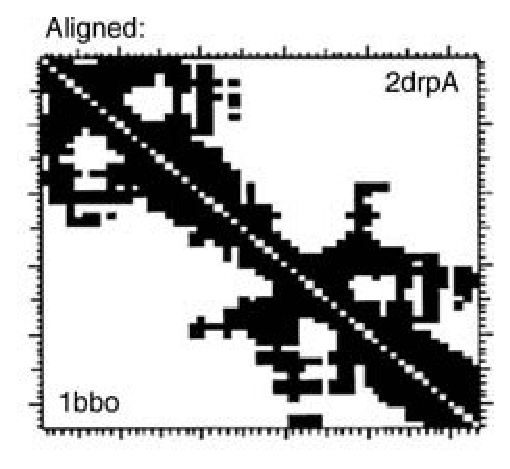
\includegraphics{dali}
%\caption%[]
%{
%Alineamiento DALI de matrices de contactos/distancias, tomado de \cite{Holm2006}. 
%Estas matrices se pueden calcular por ejemplo con RRDistMaps, 
%que es parte de \htmladdnormallink{CHIMERA}{http://rbvi.ucsf.edu/chimera/download.html}.
%}
%\label{fig:dali}
%\end{center}
%\end{figure}

\begin{figure}
\begin{center} 
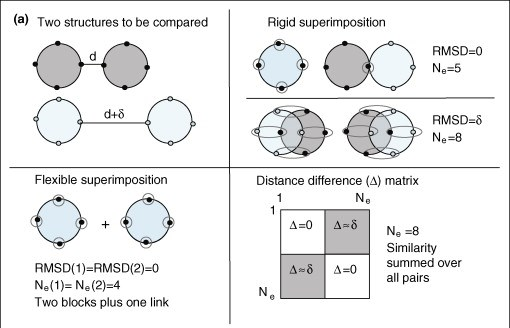
\includegraphics{3Dsuper}
\caption%[]
{
Tres estrategias (r\'{i}gida, flexible y el\'{a}stica) para comparar la estructura terciaria de dos prote\'{i}nas 
con dos dominios (c\'{i}rculos) con 4 residuos cada uno, separados por una secuencia de longitud variable.
Arriba derecha: la superposici\'{o}n r\'{i}gida tiene dos opciones: alinear un total de 5 residuos equivalentes ($Ne$) con RMSD bajo 
o alinear todos ($Ne=8$) con un RMSD alto. 
Abajo izquierda: una superposici\'{o}n flexible rompe la estructura larga en dos subestucturas para optimizar el RMSD sobre 4 residuos en cada dominio.
Abajo derecha: la comparaci\'{o}n de matrices de distancias permite alinear ambos dominios maximizando $Ne$.
Figura tomada de \citet{Hasegawa2009} y reproducida con permiso.
}
\label{fig:dali}
\end{center}
\end{figure}


\begin{figure}
\begin{center} 
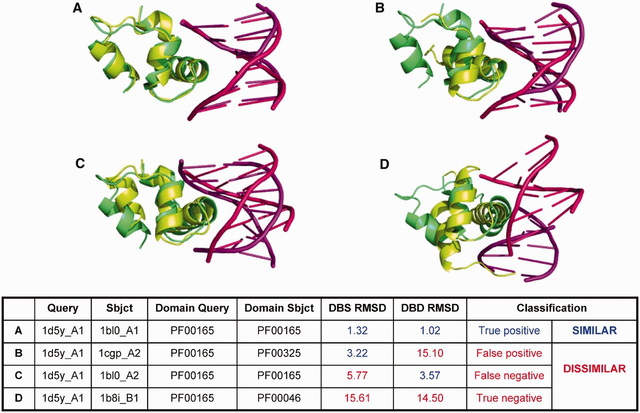
\includegraphics{tfcompare}
\caption%[]
{
Superposiciones de dominios de uni\'{o}n a DNA (DBD) de factores de transcripci\'{o}n, que ponen de manifiesto 
su mecanismo, no siempre conservado, de reconocimiento de sus cis-elementos (DBS). 
Figura tomada de \citet{Sebastian2013}.
}
\label{fig:tfcompare}
\end{center}
\end{figure}

Hay disponibles muchos otros programas disponibles para la comparaci\'{o}n estructural de prote\'{i}nas, 
y cada usuario tiene el suyo preferido. A qu\'{e} se debe esto? 
La raz\'{o}n es que no existe una definici\'{o}n totalmente satisfactoria del alineamiento estructural correcto, 
que es en definitiva la funci\'{o}n que todos estos algoritmos tratan de optimizar. De hecho, ni siquiera
est\'{a} claro si las taxonom\'{i}as estructurales cl\'{a}sicas, 
como \htmladdnormallink{CATH}{http://www.cathdb.info} o
\htmladdnormallink{SCOP}{http://scop.berkeley.edu} \citep{Csaba2009},
son compatibles con la evidencia disponible sobre la evoluci\'{o}n de los plegamientos (\italics{folds}), que
actualmente se imagina como un proceso discreto s\'{o}lo hasta cierto punto \citep{Taylor2002,Pascual2009,Sadowski2010,Andreeva2014}. 
De hecho \htmladdnormallink{SCOP2}{http://scop2.mrc-lmb.cam.ac.uk/} se hizo para superar esas limitaciones.
Otra complicaci\'{o}n adicional es que algunos plegamientos pueden verse como permutaciones circulares de elementos de estructura 
secundaria de otros \citep{Schmidt-Goenner2010}.

A pesar de estas dificultades, en general aceptamos que cada superfamilia de prote\'{i}nas es un \textbf{cl\'{u}ster}
de estructuras muy similares, que se pueden superponer aunque su secuencia sea muy diferente, 
y que cada plegamiento es un subconjunto de superfamilias que comparten una topolog\'{i}a de estructura secundaria.

Lo habitual cuando se publica un nuevo m\'{e}todo es compararlo con otros preexistentes. Estas comparaciones, 
si son rigurosas y reproducibles, pueden ayudar en la tarea de seleccionar un programa id\'{o}neo 
para esta tarea. El algoritmo MAMMOTH, con el que vamos a trabajar, se resume en estos pasos, 
en palabras textuales de sus autores \citep{Ortiz2002}:
\begin{quote}
 1.- From the Calpha trace,  compute the unit-vector  U-RMS  between
 all pairs of heptapeptides of both model and experimental structure.
 The  U-RMS is  described  in:  Kedem, Chew & Elber  (1999)  Proteins
 37(4):554-64,  and  in  Chew, Huttenlocher, Kedem & Kleinberg (1999)
 J.Comp.Biol. 6, 313-325.  This is a measure sensitive  to  the local
 structure.

  2.- Use the matrix derived in step 1 to find and alignment of local
 structures that maximizes the local similarity of both the model and
 the  experimental structure. For that, use a global alignment method 
 with  zero  end  gaps,  as  described  in  Needleman & Wunsch (1970) 
 J.Mol.Biol. 48, 443-453.

  3.- Find the maximum subset of similar  local  structures that have
 their corresponding  Calphas  close  in  cartesian space. "Close" is
 considered here  as  a distance less or equal than 4.0 A. The method
 to  find this subset is a small variant of the MaxSub algorithm from
 the  Fischer  group:  Siew,  Elofsson,  Rychlewski  & Fischer (2000)
 Bioinformatics, in press.

  4.- Obtain  the  probability  of  obtaining the given proportion of
 aligned residues (with respect to the  shortest  protein  model)  by
 chance.  This  metric  (E-value) is then used as the final score (or 
 the  corresponding Z-score, both are equivalent for gaussian distri-
 butions, however the Z-score is a more manegable index). In order to
 obtain this  value, an approach similar to that of Levitt & Gerstein 
 (1998) PNAS 95, 5913 is used, as  described  in  Abagyan  &  Batalov 
 (1997) J.Mol.Biol. 273, 355-368.  The E-value estimation is based on
 extreme-value fitting.  In  a  test  set  with the SCOP database, it 
 shows rather good performance.
\end{quote}
 
MAMMOTH fue comparado con varios m\'{e}todos, como se ve en esta figura:  

\begin{figure}
%\htmlimage{scale=0.5}
\begin{center} 
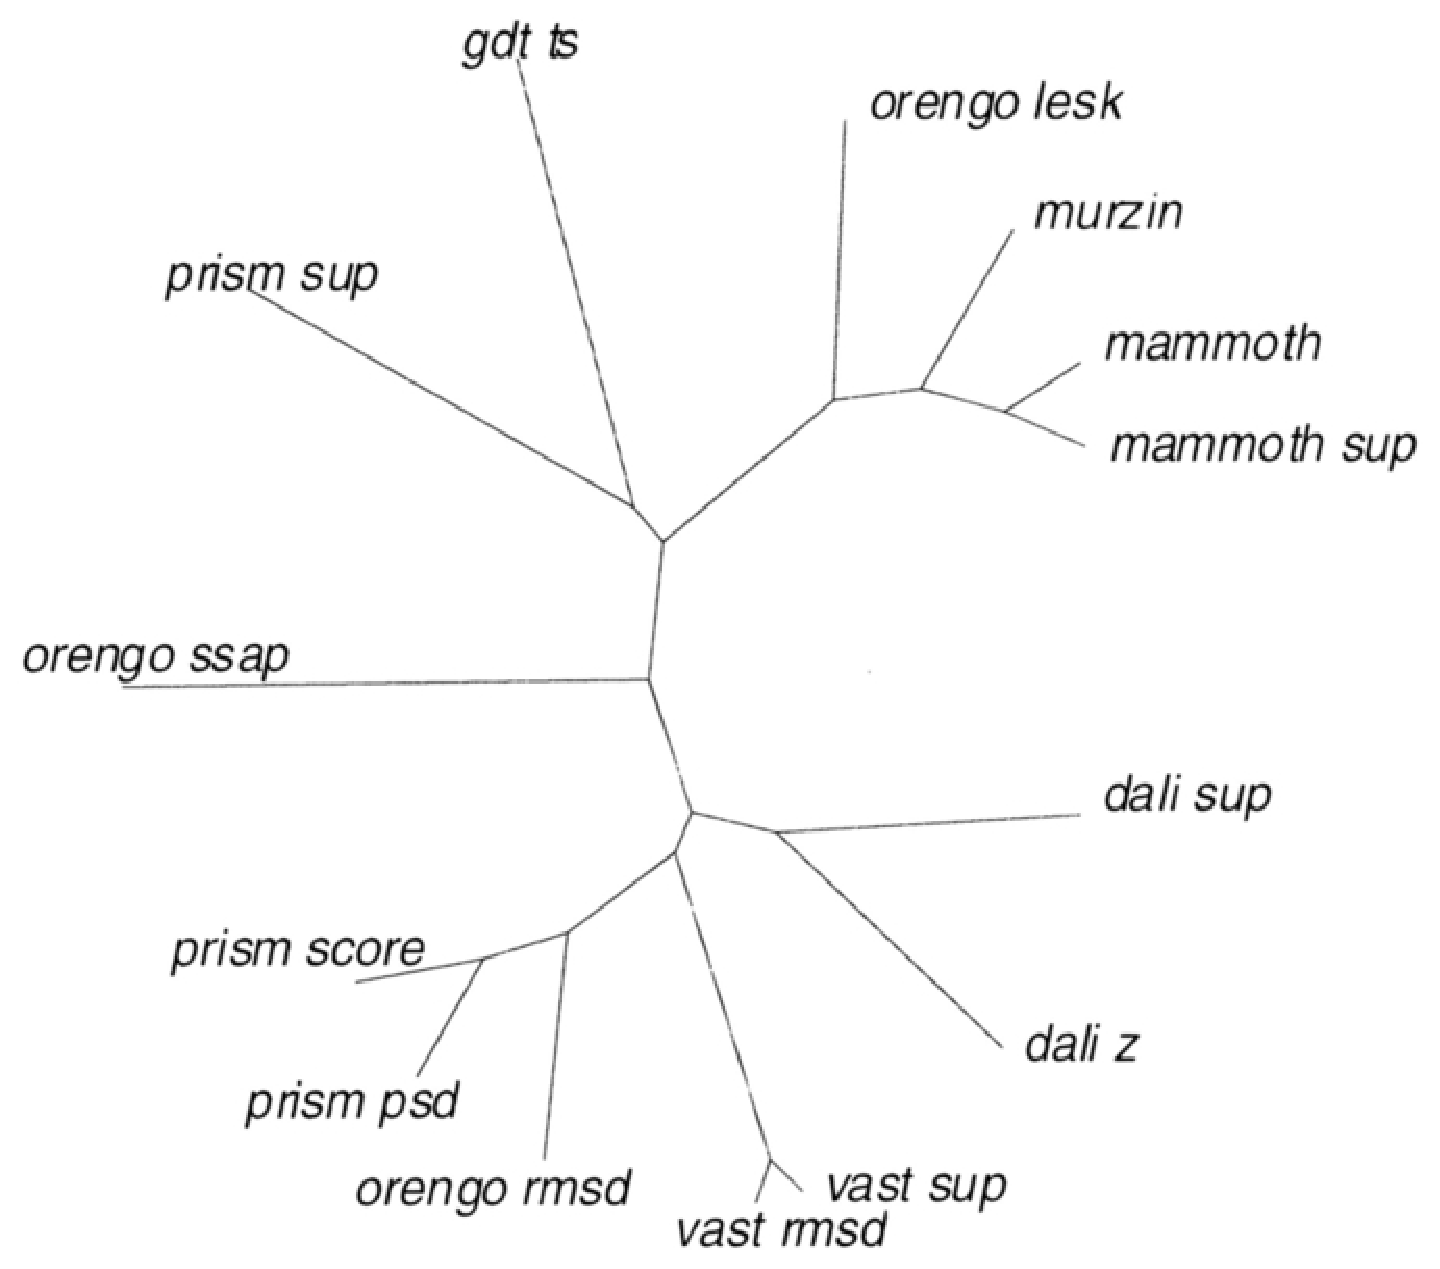
\includegraphics{mammoth_bench}
\caption%[]
{
Semejanza de MAMMOTH respecto a otros algoritmos de comparaci\'{o}n de estructura de prote\'{i}nas, 
incluyendo el criterio de un experto humano (Murzin). Figura tomada de \citet{Ortiz2002}. Copyright (2002) Protein Science.
}
\label{fig:mammoth}
\end{center}
\end{figure}
%$https://www.ncbi.nlm.nih.gov/pmc/articles/PMC2373724/

MAMMOTH es junto con DALI de los mejores programas, porque adem\'{a}s de generar superposiciones y alineamientos satisfactorios, 
sus medidas num\'{e}ricas de similitud devuelven valores que se ajustan a la evaluaci\'{o}n visual de la superposici\'{o}n obtenida.
En concreto, MAMMOTH devuelve para cada alineamiento una puntuaci\'{o}n y su valor esperado asociado (\italics{E-value}),
que podemos interpretar de manera an\'{a}loga a los valores esperados de BLAST, superando las limitaciones del RMSD para 
comparar estructuras que solamente se parecen en algunas regiones \citep{Siew2000}. 
Adem\'{a}s, hay una versi\'{o}n de MAMMOTH que permite calcular 
\htmladdnormallink{alineamientos m\'{u}ltiples}{https://ub.cbm.uam.es/software/mammothm.php}.

Para superar las limitaciones del RMSD, que da el mismo peso a regiones del core que a regiones divergentes, 
\citet{Zhang2004} propusieron otra funci\'{o}n, el TM-score, que disminuye el peso de las parejas alineadas a mayor distancia, es menos sensible
a la longitud de las estructuras comparadas y toma valores entre 0 y 1: 

\begin{equation}
TMscore = max[  \frac{1}{L_{Q}}  \sum_{i=1}^{L_{T}} \frac{1}{ 1 + (\frac{d_{i}}{d_{0}})^{2} } ]
\end{equation} 

Aqu\'{i} $max$ es el valor m\'{a}ximo obtenido en todas las superposiciones calculadas, 
$L_{Q}$ es la longitud de la estructura Q o \italics{query}, 
$L_{T}$ es el total de residuos alineados a la estructura T o \italics{template}, 
$d_{i}$ es la distancia entre la pareja $i$ de residuos y 
$d_{0}$ el factor de escala para normalizar por longitud de secuencia. 

Para calcularlo de manera \'{o}ptima podemos usar su algoritmo TM-align \citep{Zhang2005}, cuyo c\'{o}digo fuente esta disponible en 
\htmladdnormallink{TMalignc.tar.gz}{http://zhanglab.ccmb.med.umich.edu/TM-align/TM-align-C/TMalignc.tar.gz}. La funci\'{o}n TM-score
se ha convertido en el est\'{a}ndar para medir el parecido entre estructuras, ya que se acepta que un valor de 0.5 garantiza un plegamiento similar.

De todos modos, hay una gran variedad de software para esta tarea, 
como se muestra por ejemplo en esta \htmladdnormallink{lista de la WikipediA}{http://en.wikipedia.org/wiki/Structural_alignment_software}.

%\subsection{Ejercicios de similitud estructural entre estructuras proteicas con MAMMOTH}
Para aprender a hacer alineamientos/superposiciones estructurales, y a interpretarlos, podemos hacer este ejercicio:

\begin{itemize}

\item Visita \htmladdnormallink{SCOPe}{http://scop.berkeley.edu}, 
elige una clase (ver figura \ref{fig:foldclassif})
%elige la opci\'{o}n \italics{Enter SCOP at the top of the hierarchy} 
y selecciona un grupo de 5 estructuras de prote\'\i{}nas que pertenezcan a la misma superfamilia, para despu\'{e}s
\begin{itemize}
\item descargar los archivos PDB correspondientes,que contienen las coordenadas at\'{o}micas,  del
\htmladdnormallink{Protein Data Bank}{http://www.rcsb.org/pdb} y
\item compara al menos una pareja de estructuras con MAMMOTH %\htmladdnormallink{MAMMOTH}{https://ub.cbm.uam.es/software/mammoth.php} 
e inspecciona los archivos de salida generados (\verb+maxsub_sup.pdb,maxsub_sup2.pdb,rasmol.tcl+)
%o con la versi\'{o}n \htmladdnormallink{web}{https://ub.cbm.uam.es/software/online/mammoth.php})
\item (el ejecutable se encuentra en \verb+/home/compu2/algoritmos3D/soft/mammoth-1.0-src+)
\end{itemize}
 
\item Visualiza la superposici\'{o}n generada,  con Rasmol (usando la opci\'{o}n \verb+ -script rasmol.tcl+) y con PyMOL

\item Puedes probar a superponer estructuras directamente en \htmladdnormallink{PyMOL}{https://pymol.org/dokuwiki/doku.php?id=command:align}

\item Prueba MAMMOTH con el fin de comparar una estructura problema (una de las 5) contra una biblioteca
de estructuras en formato PDB (las otras 4), como si fuera BLAST. Cu\'{a}l de las 4 estructuras ser\'{i}a el mejor molde o \italics{template})
Cu\'{a}l es el l\'{i}mite esperado de precisi\'{o}n, en t\'{e}rminos de RMSD, que alcanzar\'{i}amos con cada molde?

\item Calcula para algunas de las superposiciones el \htmladdnormallink{TM-score}{http://zhanglab.ccmb.med.umich.edu/TM-score/}.

%Por ejemplo puedes comparar la luciferasa bacteriana 
%\htmladdnormallink{LuxA}{http://www.rcsb.org/pdb/explore/explore.do?structureId=1LUC} con las entradas de la
%biblioteca que puedes descargar de este \htmladdnormallink{enlace}{./files/scoplibrary.tgz} (3.7Mb).
\end{itemize}
